% This document is compiled using pdfLaTeX
% You can switch XeLaTeX/pdfLaTeX/LaTeX/LuaLaTeX in Settings

\documentclass[b5paper, twoside]{article}
\usepackage{ctex}
\usepackage{csquotes} % 对于智能引用符号
\usepackage[backend=biber,style=numeric]{biblatex} % 使用biblatex和biber
\usepackage{geometry}
\usepackage{graphicx}
\usepackage{listings}
\usepackage{minted}
\usepackage{amsmath}
\usepackage{amsfonts}
\usepackage[T1]{fontenc}
\usepackage{lmodern}
\usepackage{amssymb}
\usepackage{marginnote}
\usepackage{xcolor}
\usepackage{hyperref}
\usepackage{todonotes}
\usepackage[utf8]{inputenc}
\usepackage{mdframed}
\usepackage{multicol}
\usepackage{url} % 加载url包
\usepackage[linesnumbered,ruled,vlined]{algorithm2e}
\usepackage{array} % 提供>{...}功能
\usepackage{booktabs} % 提供更好的表格线条
\usepackage{lipsum} % 用于生成占位文本
\usepackage{titlesec}
\usepackage{titling}
\usepackage{wrapfig}
\usepackage{enumitem}
\usepackage{parskip}
\usepackage{graphicx}
\usepackage{tikz}

\fvset{breaklines=true,
    frame=lines
}
\setlength{\parskip}{0pt}    % 设置段落之间的间距
\setlist[itemize,1]{left=0pt}
\setlist[itemize,2]{left=1pt}
\setlist[itemize,3]{left=1pt}
% 定义一个命令来设置图片的透明度
\let\oldincludegraphics\includegraphics
\renewcommand{\includegraphics}[2][]{%
  \begin{tikzpicture}
    \node[opacity=0.7] {\oldincludegraphics[#1]{#2}};
  \end{tikzpicture}%
}
% 设置页边距
\geometry{
    left=2cm,         % 左边距
    right=2cm,        % 右边距
    top=2.5cm,          % 上边距
    bottom=2.5cm        % 下边距
}
\lstset{
  language=Python,      % 语言类型
  basicstyle=\tt, %使用teletype字体
}
% 定义蓝色
\definecolor{myblue}{RGB}{0, 100, 225}
% 重新定义 \maketitle 命令
\pretitle{\begin{center}\LARGE\bfseries\color{blue}}
\posttitle{\end{center}}
% 重定义 \textbf 命令
\let\oldtextbf\textbf
\renewcommand{\textbf}[1]{\textcolor{myblue}{\oldtextbf{#1}}}
\titleformat{\section}
  {\color{myblue}\bfseries\Large}
  {\thesection}
  {1em}
  {}
\titleformat{\subsection}
  {\color{myblue}\bfseries\large}
  {\thesubsection}
  {1em}
  {}
\titleformat{\subsubsection}
  {\color{myblue}\bfseries\normalsize}
  {\thesubsubsection}
  {1em}
  {}
% 定义一个带有较小字体的 mdframed 环境
\newenvironment{smallmdframed}
  {\begin{mdframed}[linewidth=0pt, backgroundcolor=pink!20]\small}
  {\end{mdframed}}
  
\title{数据库系统笔记：SYSU2022人工智能学院课程}
\date{}

\begin{document}
\begin{minipage}[t]{\textwidth}
    \vspace{-0.5cm}
    \begin{center}
        \vspace{-1.5cm} % 减少间距
        
\includegraphics[width=0.2\textwidth]{sysu.jpg}\\
        \vspace{-1.5cm} % 减少间距
    \end{center}
    \maketitle
    \vspace{-4cm} % 减少间距
\end{minipage}
\vspace{-0.8cm}

\section*{9. 关系型数据库设计：3NF}
数据库异常行为包括函数依赖下的冗余存储、异常更新、异常插入、异常删除，如下图（position$\rightarrow$salary）。
\begin{figure}[ht]
  \centering
  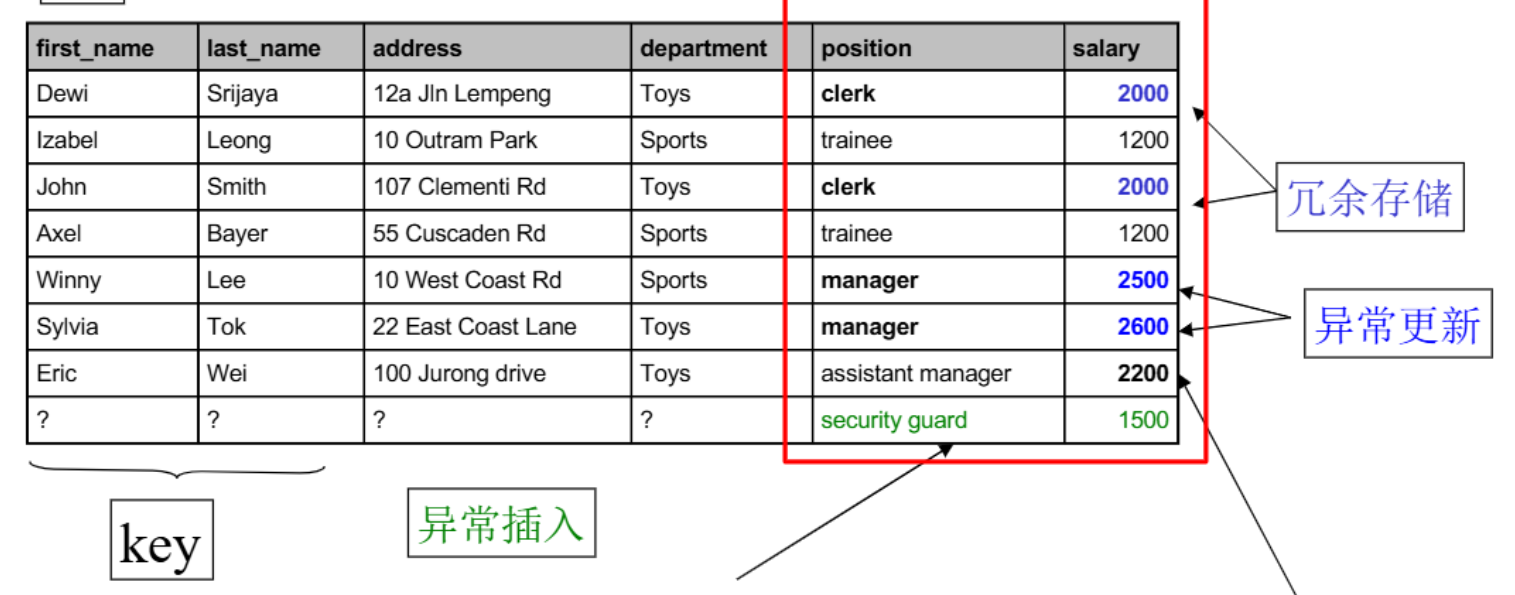
\includegraphics[width=0.8\linewidth]{img/屏幕截图 2024-11-04 112858.png}
  \caption{数据库异常行为}
  \label{fig:my_label}
\end{figure}

\textbf{规范化}是将关系型数据库分解的过程。$\mathbf{R}=R_1, R_2, \dots, R_n$。
\begin{itemize}
    \item 要求分解无损、依赖保留且冗余信息小。
\end{itemize}

\textbf{依赖保留}：FDs存在于各个单个relation，以便于验证FD。
\begin{itemize}
    \item 即，所有子表格FD并集的闭包与原来表格FD闭包一致
\begin{smallmdframed}
    给定一组函数依赖 $F$，$F$ 的闭包记作 $F^+$，它是所有由 $F$ 逻辑上蕴涵的函数依赖的集合。换句话说，$F^+$ 包括 $F$ 中的所有函数依赖以及可以通过 $F$ 中的函数依赖使用推理规则推导出来的所有函数依赖。

    计算一个属性集 $X$ 关于一组函数依赖 $F$ 的闭包 $X^+$ 的方法如下：

    \begin{enumerate}
    \item \textbf{初始化}：设 $X^+$ 为 $X$ 的初始值。
    \item \textbf{迭代}：重复以下步骤直到 $X^+$ 不再变化：
        \begin{itemize}
            \item 对于每一个 $F$ 中的函数依赖 $A \rightarrow B$，
                \begin{itemize}
                    \item 如果 $A \subseteq X^+$，则将 $B$ 添加到 $X^+$ 中。
                \end{itemize}
        \end{itemize}
    \end{enumerate}

    当 $X^+$ 不再变化时，算法结束，此时 $X^+$ 就是 $X$ 在 $F$ 下的闭包。
\end{smallmdframed}
\end{itemize}

\textbf{不满足依赖保留的分解：}
\begin{itemize}
    \item 可能会出现信息丢失、存储冗余等问题。
    \item 如果不能通过自然连接而恢复依赖，则出现信息丢失。
    \item 在下图中，$R_1$和$R_2$不存在依赖$B\rightarrow C$。
\begin{figure}[ht]
    \centering
    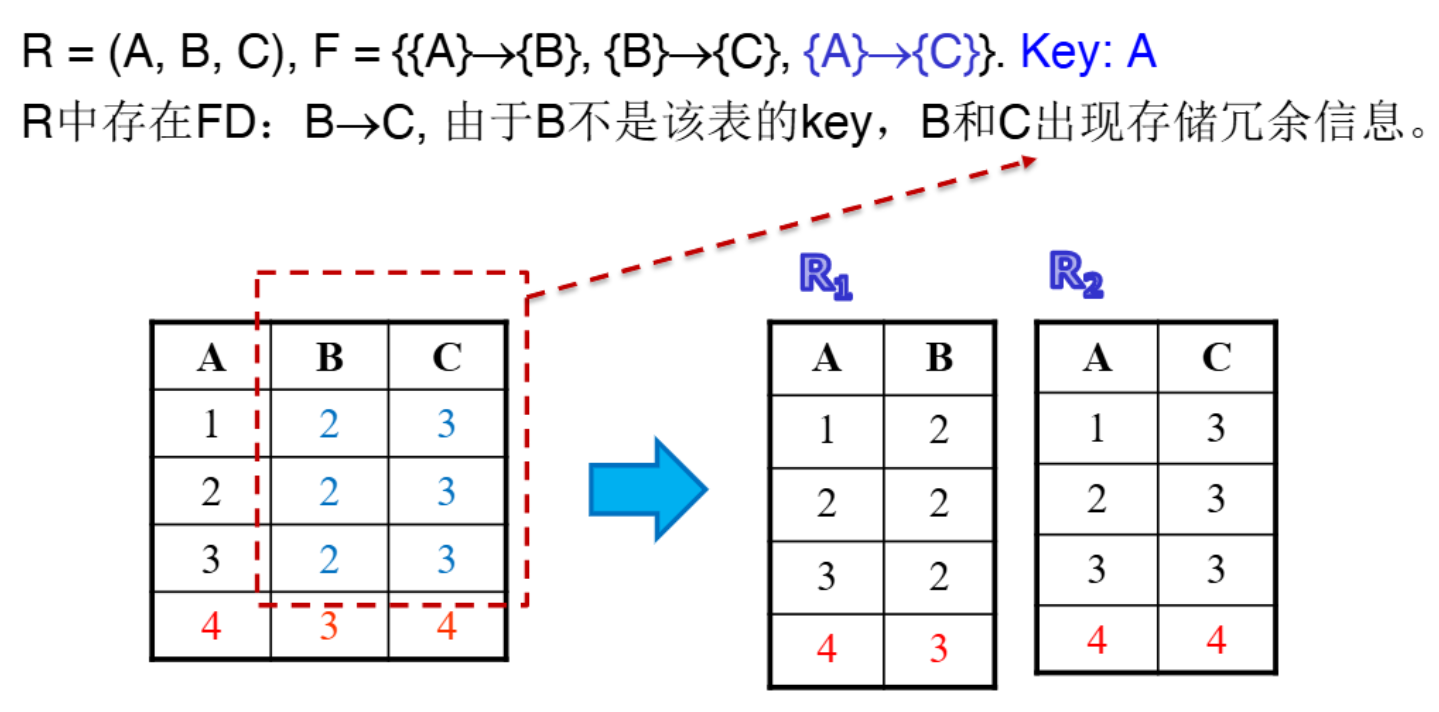
\includegraphics[width=0.7\linewidth]{img/屏幕截图 2024-11-04 134914.png}
    \label{fig:my_label}
    \caption{错误分解}
\end{figure}
    \item $F_1=\{\{A\}\rightarrow\{B\}\}\&F_2=\{\{A\}\rightarrow\{C\}\}, ({F_1}\cup{F_2})^+\neq{F}^+$。正确分解如图3。
\begin{figure}[ht]
  \centering
  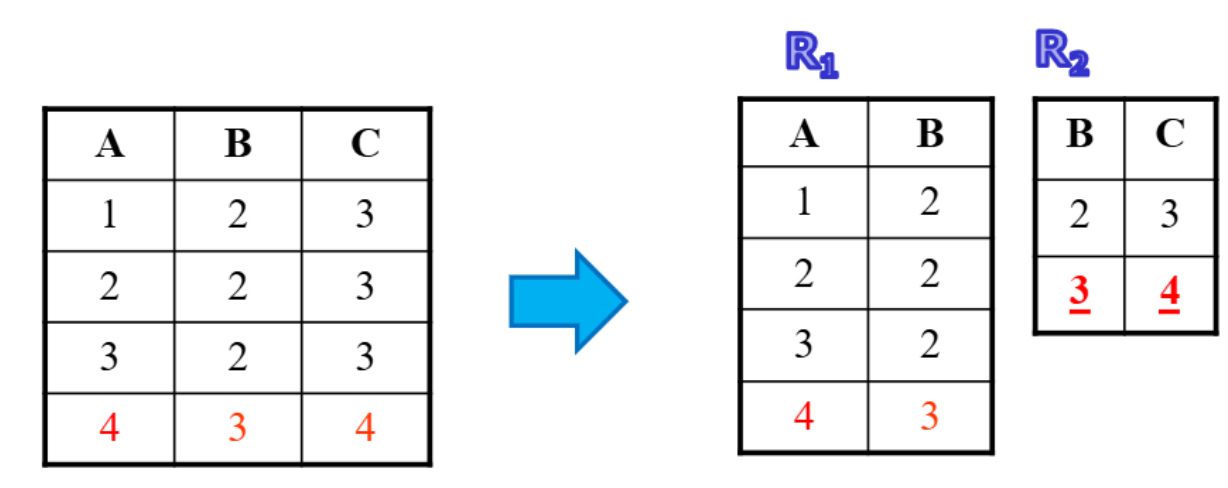
\includegraphics[width=0.6\linewidth]{img/屏幕截图 2024-11-04 141626.png}
  \caption{正确分解}
  \label{fig:my_label}
\end{figure}
\end{itemize}

\textbf{Lossless Join Decomposition：} 
\begin{itemize}
    \item 如果能利用分解后的表恢复原来的表，则该分解是无损的。
    \item 两个schema的交集属性至少构成其中一个schema的key。
    \begin{itemize}
        \item 外键必须引用另一个表的候选键。
    \end{itemize}
\end{itemize}

\textbf{1NF：第一范式}
\begin{itemize}
    \item 第一范式：表中所有属性的域没有多值属性。
    \item 根据关系模型的定义，关系表（relational tables）永远是1NF。
    \begin{itemize}
        \item 关系模型要求每一个属性都是原子的。
    \end{itemize}
\begin{smallmdframed}
1NF是不够的，不一定能满足无损、依赖保留和形式良好。
\\ 范式是对关系模式的规范化，不是对分解方法的选择。
\end{smallmdframed}
\end{itemize}

\textbf{2NF：第二范式}
\begin{itemize}
    \item 定义：1NF基础上，所有非主属性完全函数依赖于任何一个候选键。
    \begin{itemize}
        \item 2NF确保所有非主属性完全依赖于任何一个候选键，而不是部分依赖于候选键的一部分。即，非主属性必须完全依赖于候选码。
        \item 2NF通过消除部分函数依赖，可以减少数据冗余，提高数据的一致性和完整性。
    \end{itemize}
    \item 形式化：$R$ 是在 2NF 中当且仅当对于每个函数依赖 $X \rightarrow \{A\}$ 在 $F^+$ 中，至少满足以下三个条件的其中一条：
    \begin{itemize}
        \item $A \in X$（函数依赖是平凡的）：自己依赖自己，无函数依赖
        \item $X$ 不是某个候选键的真子集：被依赖属性非为部分候选键
        \item $A$ 是一个主属性
    \end{itemize}
    \item 向2NF的转换：
    \begin{itemize}
        \item 如果存在非主属性对候选码的部份依赖，则这个属性和主关键字这一部分应该分离开作为一个新表。
    \end{itemize}
\begin{smallmdframed}
假设关系模式 $R(A, B, C, D)$，$(A, B)$ 是主键，函数依赖集为 $F = \{A \rightarrow C, (A, B) \rightarrow D\}$。

\begin{itemize}
        \item 主键是 $(A, B)$。
        \item 非主属性是 $C$ 和 $D$。
        \item 函数依赖 $A \rightarrow C$ 表明 $C$ 部分依赖于主键 $(A, B)$ 的一部分 $A$。
        \item 函数依赖 $(A, B) \rightarrow D$ 表明 $D$ 完全依赖于主键 $(A, B)$。
\end{itemize}
结论：关系模式 $R$ 不满足2NF，因为存在部分函数依赖 $A \rightarrow C$。
\\转换为2NF：
\begin{itemize}
    \item 分离成为两个关系模式$R_1(A,C)$和$R_2(A,B,D)$。
    \item $R_1$和$R_2$的FDs，非主属性都完全依赖于主键。
\end{itemize}
\end{smallmdframed}
\end{itemize}


\textbf{3NF：第三范式}
\begin{itemize}
    \item 定义：在1NF的基础上，任何非主属性不依赖于非键。
    \begin{itemize}
        \item 理解：在2NF的基础上消除传递依赖。
        \item 3NF同样减少数据冗余和提高数据的一致性。
    \end{itemize}
    \item 形式化：$R$ 是在 3NF 中当且仅当对于每个函数依赖 $X \rightarrow \{A\}$ 在 $F^+$ 中，至少满足以下三个条件的其中一条：
    \begin{itemize}
        \item $A \in X$（函数依赖是平凡的）。
        \item $X$ 是R的超键。（相比起2NF的更进一步。）
        \item $A$ 是一个主属性。
    \end{itemize}
    \item 3NF的分解：假设有一个关系模式 \( R(A, B, C, D) \)，其函数依赖集为 \( F = \{A \rightarrow B, B \rightarrow C, A \rightarrow D\} \)。
    \begin{itemize}
        \item {确定候选键}：计算属性闭包，发现 \( A \) 是候选键，因为 \( A^+ = \{A, B, C, D\} \)。
        \item {识别非主属性}：非主属性是 \( B \)、\( C \) 和 \( D \)。
        \item {检查传递依赖}：存在传递依赖 \( A \rightarrow B \rightarrow C \)，因为 \( A \rightarrow B \) 且 \( B \rightarrow C \)，但 \( A \not\rightarrow C \)。
        \item {分解关系模式}：将 \( R \) 分解为两个关系模式：\( R_1(A, B, D) \)和\( R_2(B, C) \)
    \end{itemize}
\begin{smallmdframed}
    一个值得注意的自环传递例子：
    \begin{itemize}
        \item $R=(B,C,E)$，$F = \left\{ \{{E}\} \to \{{B}\}, \; \{{B,C}\} \to \{{E}\} \right\}$
        \item 找出候选键：BC和EC。
        \item 满足任何非主属性不依赖于非键。
        \item 该关系模式符合3NF范式。
    \end{itemize}
\end{smallmdframed}
\end{itemize}

\textbf{BCNF：Boyce-Codd范式}
\begin{itemize}
    \item BCNF旨在消除非平凡的多值依赖和非主属性对候选键的部分依赖。
    \item 形式化：$R$ 是在 BCNF 中当且仅当对于每个函数依赖 $X \rightarrow \{A\}$ 在 $F^+$ 中，至少满足以下三个条件的其中一条：
    \begin{itemize}
        \item $A \in X$（函数依赖是平凡的）。
        \item $X$ 是R的超键。
    \end{itemize}
    \item （$\dots$）
\end{itemize}

\section*{10. 内存层级和文件组织$_{377}$}

\section*{11. 索引$_{405}$}

\textbf{索引的概念和引入}
\begin{itemize}
    \item 索引的评估：成本定义为最坏情况下的磁盘打开页数。
    \item ID排序+二分搜索：$\log(n)$。
    \item ID排序+索引条目：$<ID, page.No>$\lstinline{[Search-key|pointer]}
    \begin{itemize}
        \item 每个page的第一条记录有一个条目，从而反映条目区间。
        \item 对索引使用二分查找。
        \item 可以创建多级索引Multilevel Index。
    \end{itemize}
    \item 两种基础索引类型：顺序索引、哈希无序索引。
\end{itemize}

\textbf{顺序索引}
\begin{itemize}
    \item 顺序索引也成为树索引。
    \item 获取一个记录所需的page访问次数为\lstinline{tree.height+1}
\begin{figure}[ht]
  \centering
  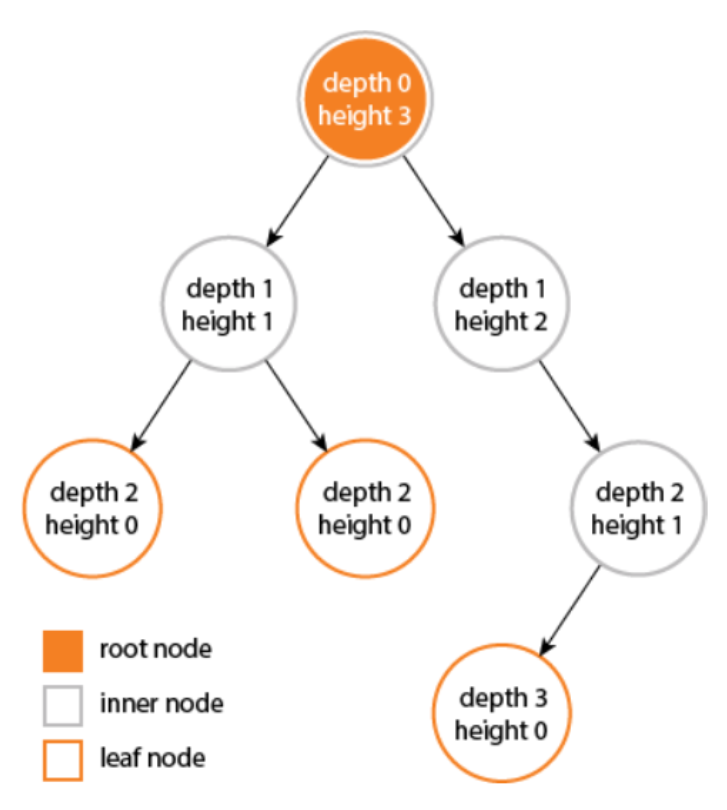
\includegraphics[width=0.3\linewidth]{img/屏幕截图 2024-11-05 142036.png}
  \caption{tree index}
  \label{fig:my_label}
\end{figure}
    \item 主索引和辅助索引：
    \begin{itemize}
        \item 主索引{Primary index}：文件实际存放也是按照search key 排序的。其基于主键或唯一标识符构建索引，具有唯一性。
        \item 辅助索引{Secondary index}：也称为二级索引。文件的实际存放不按照search key 排序。其基于非主属性构建索引，不具有唯一性。
        \\ 1. 当检索许多记录时，辅助索引昂贵，因为磁盘不连续寻址耗时长。
        \\ 2. 辅助索引常用于优化不涉及主键的查询。
    \end{itemize}
\begin{smallmdframed}
        对于非排序属性（如账号、余额等），可以通过额外建立索引生成二级索引，从而提高查询效率。这样可以在不需要重新组织数据的情况下，实现对这些属性的有效查询。
\end{smallmdframed}
    \item 稀疏索引和密集索引
    \begin{itemize}
        \item 稀疏索引Sparse Index：仅包含某些search key。
        \\稀疏检索：找到最后一个比K小key的index，然后向后遍历寻找K。
        \item 密集索引Dense Index：包含所有search key。
        \begin{figure}[ht]
            \centering
            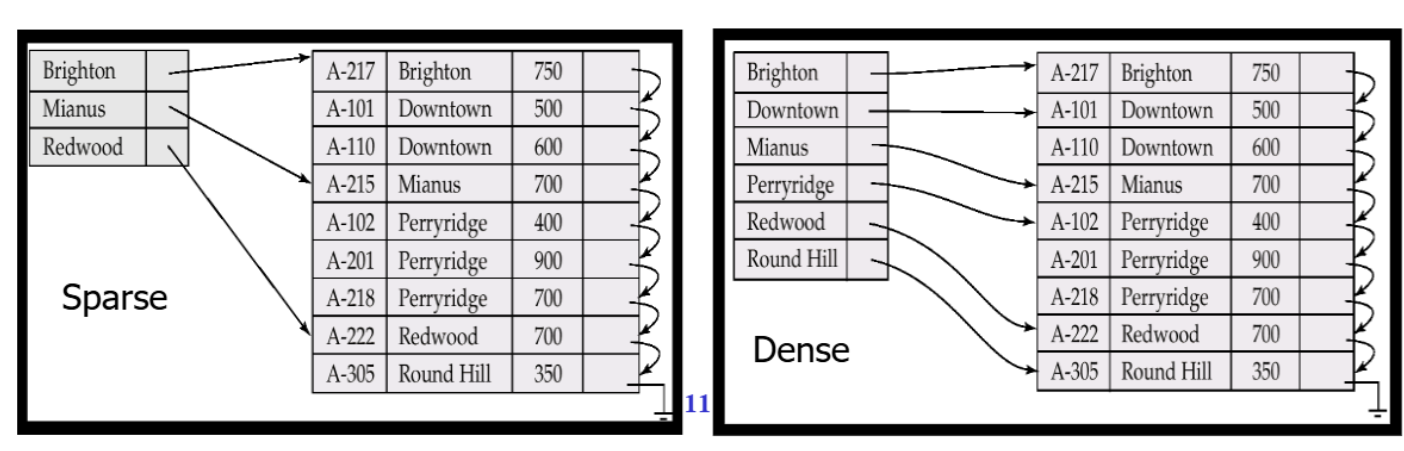
\includegraphics[width=0.7\linewidth]{img/image.png}
            \caption{稀疏索引和密集索引}
            \label{fig:my_label}
        \end{figure}
    \end{itemize}
\end{itemize}

\textbf{哈希索引}
\begin{figure}[ht]
  \centering
  \begin{minipage}[b]{0.45\textwidth}
    \centering
    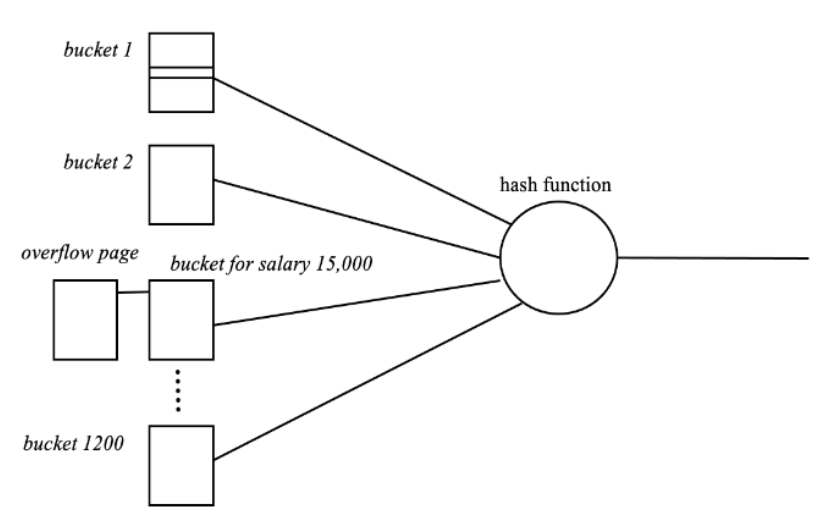
\includegraphics[width=\linewidth]{img/屏幕截图 2024-11-05 160116.png}
    \caption{哈希索引结构}
    \label{fig:hash_structure}
  \end{minipage}%
  \hfill
  \begin{minipage}[b]{0.45\textwidth}
    \centering
    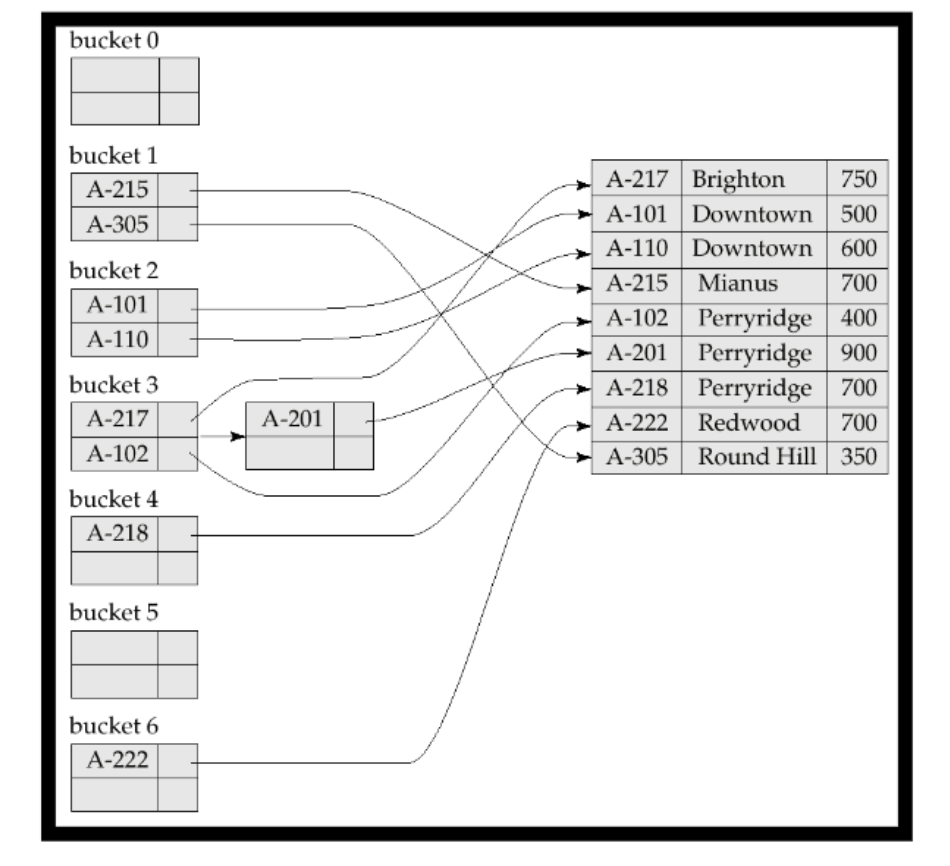
\includegraphics[width=0.8\linewidth]{img/屏幕截图 2024-11-05 161453.png}
    \caption{哈希索引示例}
    \label{fig:hash_example}
  \end{minipage}
\end{figure}
\begin{itemize}
    \item 哈希索引维护哈希函数\lstinline{F(search key)=location_of_record}
    \item 严格来说，哈希索引是二级索引。
\end{itemize}

\textbf{索引的评价指标}
\begin{itemize}
    \item 高效支持不同查询：例如，辅助索引（包括哈希）在范围检索表现很差，因为磁盘经常需要跨区寻址。
    \item 更新时间成本小：当文件被修改时，索引也必须更新。
    \item 额外存储成本小（即index本身的大小）：索引的大小应该比数据文件小得多。
\end{itemize}

\textbf{索引的更新}
\begin{itemize}
    \item 删除：索引的删除思路符合直觉。
    \begin{itemize}
        \item 如果删除的记录为索引的唯一记录，则对应的索引也要删除。
        \item 对于稀疏索引，如果删除记录的search key 在index存在，则将index里的的记录替换为所删除的下一条记录。如果下一条记录已经在index中存在，则直接删除。
    \end{itemize}
    \item 插入：同样符合直觉。
    \begin{itemize}
        \item 对于密集索引：如果search key没有出现在index则插入。
        \item 对于稀疏索引：
    \end{itemize}
\end{itemize}
\appendix

\section*{附录1：相关习题或代码}

\end{document}
